\section{Background}

\subsection{UPPAAL}
UPPAAL \cite{Larsen1997} is a complete tool for modeling, simulation, and verification of real-time systems. Systems can be modeled as networks of automata and timed automata. A system is composed of one or more models that consist of locations and transitions between locations. Simulation involves traversing the state space to obtain possible paths within the defined system. Simulation is used to interactively check if the system behaves as expected. Verification is realized through model-checking. In the process of verification, properties defined for the system are determined to be valid or not. If the property is found to be false, UPPAAL will produce a diagnostic trace, a path through the system that contradicts the checked property. 

UPPAAL is an appropriate tool to model a robot swarm. A robot swarm is composed of multiple uniform robots. A single robot can be modeled as a timed automaton implementing an algorithm of our choice. A system consisting of multiple uniform timed automata can be used to simulate an algorithm implementation for a robot swarm. This allows us to simulate the robot swarm and perform verification. Verification through model checking can be utilized to verify the correctness of the implementation of the algorithm as well as for the emergence of the desired behavior of the swarm.


\subsection{Timed automata in UPPAAL}
The timed automaton defined in the work of Rajeev Alur and David Dill \cite{Alur1990} is a basis for timed automata used in UPPAAL. Additionally, UPPAAL extends the Definition \ref{def:automaton} of the automaton with invariants and variables of boolean and integer type. The invariant is a progression condition on the system. It states that the system is allowed to stay in a given location only for a specified time before being forced to transition. A transition between locations can be decorated with a guard, a logical condition on the system variables, or clocks. If the logical value of the guard is true, the transition is enabled and disabled otherwise. Transitions can be associated with the synchronization action. Synchronization in UPPAAL is based on handshaking; therefore, one transition is responsible for sending the synchronization signal, and one or more transitions will wait for it. A transition that is waiting for the synchronization signal will remain disabled until the signal is received. This mechanism allows for multiple processes to synchronize their transitions. During transition, it is possible to reset clocks and assign values to variables. These clock and variable values are then used to determine the logical value of the transition guards.

\newpage
\begin{definition}[Definition of timed automaton \cite{Alur1990}]
A timed automaton is a tuple $(\Sigma, S, S_0, C, E)$ where:\\
$\Sigma$ - input alphabet;\\
$S$ - finite set of automaton states;\\
$S_0 \subseteq S$ - set of start states; \\
$C$ - finite set of clocks; \\
$E \subseteq S \times S [\Sigma \cup {\epsilon}] \times 2^C \times \Phi(C)$ - set of transitions\\\\
An edge in timed automaton is a tuple $\langle s, s', \sigma, \lambda \delta \rangle$, where:\\
$s$ - origin state;\\
$s`$ - destination state;\\
$\sigma$ - input symbol for the transition;\\
$\lambda$ - set of clocks to be reset with this transition;\\
$\delta$ - condition enabling the transition;\\
\label{def:automaton}
\end{definition}


\subsection{Modeling in UPPAAL}
To explain the process of modeling in UPPAAL we will use one of the example models described in the UPPAAL tutorial \cite{SmallTutorial2009}. The example model implements Gary L. Peterson's solution to the mutual exclusion problem \cite{Peterson1981}. Figure \ref{fig:mutex_code} presents his solution to the problem of two processes sharing access to the critical section. A critical section is a part of code that must be executed only by a single process at a time \cite{Raynal2012}.

% Pseudo-code for mutex
\begin{figure}[H]
\caption{Peterson’s mutual exclusion algorithm 
\label{fig:mutex_code}
\cite{SmallTutorial2009}, \cite{Peterson1981}}
\begin{tabular}{|p{0.5\textwidth}|p{0.5\textwidth}|}
\hline
\textbf{Process 1} & \textbf{Process 2} \\
\hline
\begin{lstlisting}[basicstyle=\ttfamily]
req1=1;
turn=2;
while(turn!=1 && req2!=0);
// critical section:
job1();
req1=0;
\end{lstlisting}
&
\begin{lstlisting}[basicstyle=\ttfamily]
req2=1;
turn=1;
while(turn!=2 && req1!=0);
// critical section:
job2();
req2=0;
\end{lstlisting}
\\
\hline
\end{tabular}
\end{figure}

\noindent
Peterson's solution of the mutual exclusion algorithm consists of two symmetrical processes. Each process requests access to the critical section and then sets a flag indicating the other process's turn to access. A process will continuously wait to access the critical section until its turn or until the other process no longer requests access. After accessing the critical section and completing the associated work, the process will indicate that it no longer requests access. This solution guarantees fairness as no process will be indefinitely denied access to the critical section.


% Mutex implementation in UPPAAL
\begin{figure}[H]
\caption{Mutex automata in UPPAAL \cite{SmallTutorial2009}}
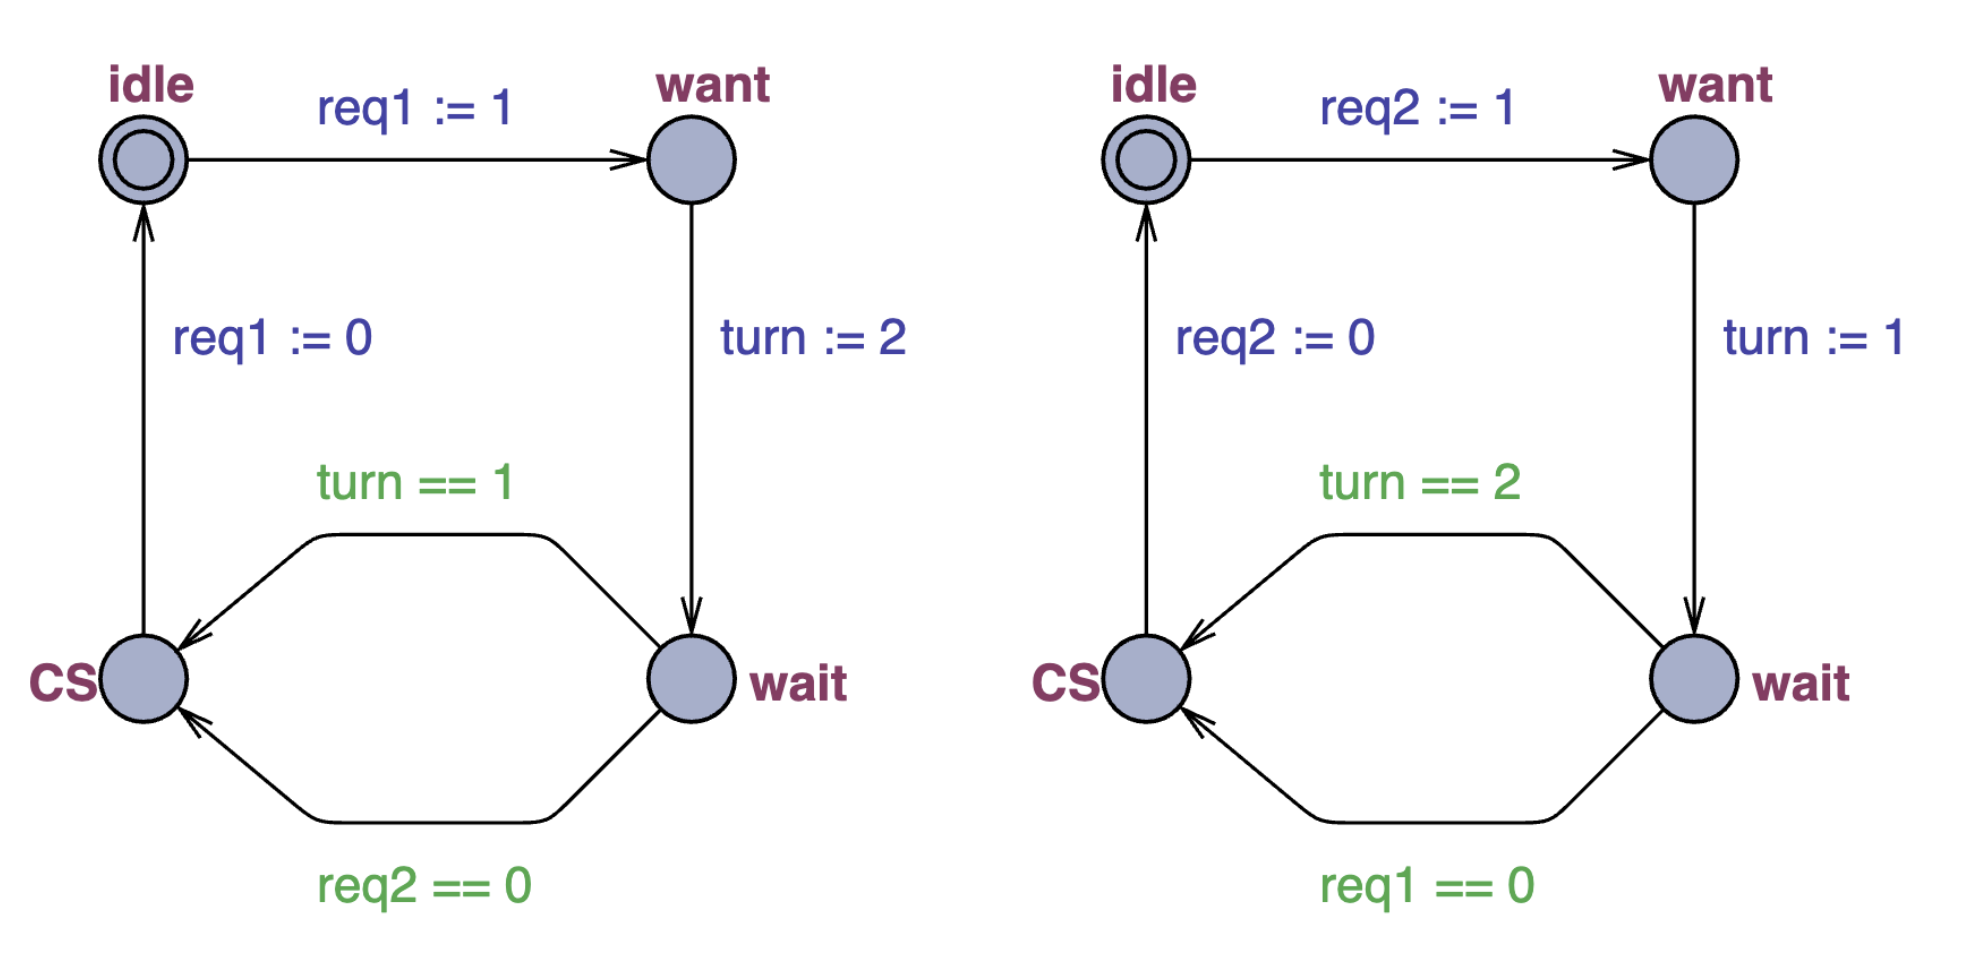
\includegraphics[width=\textwidth]{images/mutex.png}
\label{fig:mutex_uppaal}
\end{figure}

\noindent
To model Peterson's solution of the mutual exclusion algorithm we will represent two processes as separate automata. The automaton on the left in Figure \ref{fig:mutex_uppaal} will represent \texttt{Process 1} from Figure \ref{fig:mutex_code} and the right automaton will represent \texttt{Process 2}. Both automata have the same set of locations, namely, \texttt{idle}, \texttt{want}, \texttt{wait}, and \texttt{CS}. Location \texttt{idle} represents the state of the process in which it does not request access to the critical section. Location \texttt{want} represents the state of the process after requesting access to the critical section. Location \texttt{wait} indicates that the process set the turn to access the critical section to the other process. Automaton will remain in location \texttt{wait} until one of the guard conditions gets satisfied and enables the transition to location \texttt{CS}. Location \texttt{CS} is a critical section of the process. Upon transition from location \texttt{CS} to \texttt{idle} a process will no longer request access to the critical section. 


\subsection{Verifying properties in UPPAAL}
A subset of timed computation tree logic is used to express properties of the system that are verified by UPPAAL's model checking engine \cite{Bengtsson2004}. The system of timed automata is unfolded into a tree with states and transitions. Paths of such a tree are traversed by the model checking engine to determine whether defined system properties are true. System properties must be specified using logical quantifiers presented in Definition \ref{def:quantifiers}. Letters \texttt{A} and \texttt{E} are used to quantify over paths while symbols \texttt{[]} and \texttt{<>} are used to quantify over states within a path. Letter \texttt{A} is used to express property that has to hold for all paths and letter \texttt{E} is used for property that holds for at least one path. Analogically, symbol \texttt{[]} is used to express that all states within a path must satisfy the property, and symbol \texttt{<>} is used to express that there is at least one state within the path that satisfies the property.

% Logical quantifiers in UPPAAL
\begin{definition}[Logical quantifiers in UPPAAL \cite{Bengtsson2004}]
The formulas should be one of the following forms\\
- \texttt{A[]$\phi$} -- Invariantly $\phi$.\\
- \texttt{E<> $\phi$} -- Possibly $\phi$.\\
- \texttt{A<> $\phi$} -- Always Eventually $\phi$.\\
- \texttt{E[] $\phi$} -- Potentially Always $\phi$.\\
- \texttt{$\phi$ --> $\psi$} -- $\phi$ always leads to $\psi$.\\
where $\phi, \psi$ are local properties that can be checked locally on a state, i.e. boolean expressions over predicates on locations and integer variables, and clock constraints.
\label{def:quantifiers}
\end{definition}

\noindent
To present the verification process in UPPAAL we specified and successfully verified properties of Mutex implementation in Figure \ref{fig:mutex_verification}. The first property states that for all paths and all states of those paths, there is never a situation where both automata are accessing the critical section at the same time. This is a safety property that verifies whether mutual exclusion, the main objective of the algorithm, is achieved. The second and third properties are liveness properties. They state that there exists a path with a state which enables a process to access a critical section. Successful verification of all three properties means that the solution guarantees mutual exclusion and fairness. Fairness in this context means that there exists a path through the system which results in a process accessing the critical section.

% Successfully verified properties for mutex
\begin{figure}[H]
\caption{Successfully verified properties for mutex \cite{SmallTutorial2009}}
\label{fig:mutex_verification}
\begin{lstlisting}[style=code]
A[] not (P1.CS and P2.CS)
E<> P1.CS
E<> P2.CS
\end{lstlisting}    
\end{figure}